\documentclass[UTF8]{ctexbeamer}
\usefonttheme[onlymath]{serif}
\usepackage{listings}  
\usepackage{fontspec}  
\setmonofont{Consolas}  
\usepackage{graphicx}
\usepackage{amsmath}
\usetheme{metropolis}           % Use metropolis theme
\title{ODFM频域模型验证}
\date{\today}
\author{李昊}
\institute{通信系统仿真大作业}
\begin{document}
  \maketitle
  \section{整体框架}
  \begin{frame}{整体框架--流程描述}
	\begin{figure}
	  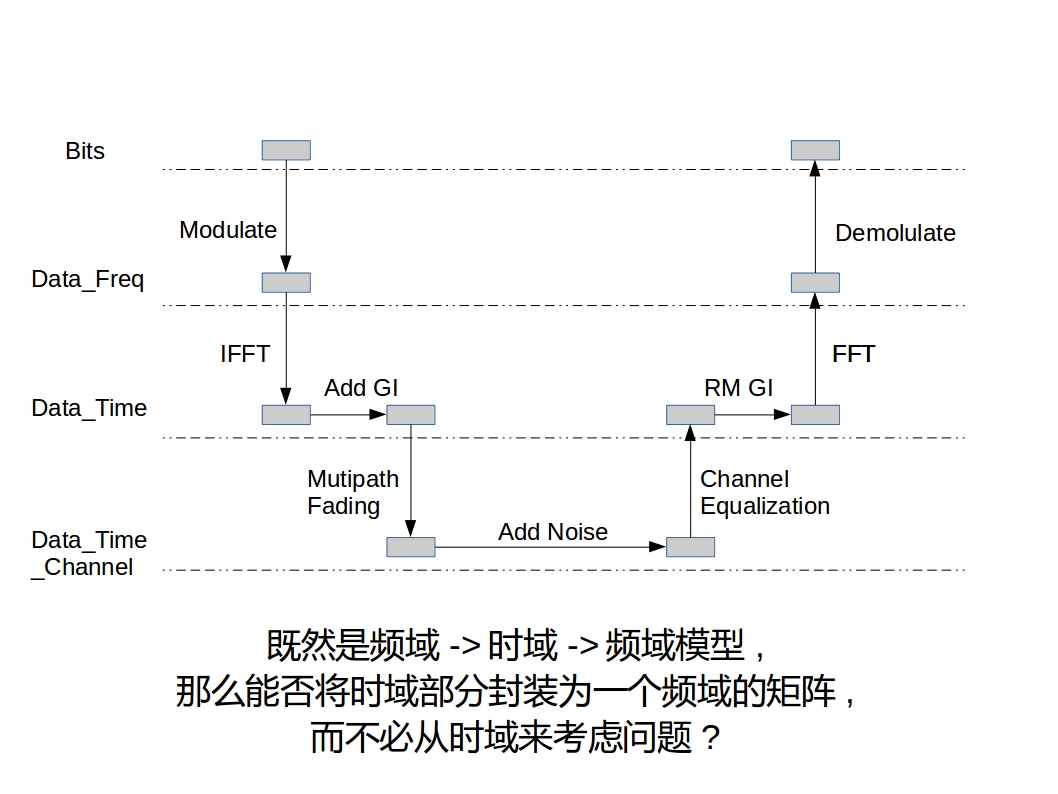
\includegraphics[width=\textwidth]{figure/top.jpg}
	\end{figure}
  \end{frame}
  \begin{frame}{整体框架--数学描述}
	\begin{equation*}
	  \begin{aligned}
	\hat Y &= FHF^{-1}X+FW \\
	 Y &= \hat Y * \frac{H_0^*}{||H_0||^2}\\
	 H_0 &= \frac{P_{Re}}{P_{Tr}} \\
	  \end{aligned}
	\end{equation*}
  \end{frame}

  \section{数字实现}
  \begin{frame}{数字实现---信道矩阵}
	\\方法一:加循环前缀和循环延时
	\scalebox{0.5}{ 	\begin{equation*}
	  \begin{aligned}
		HX &= \\ &
		\begin{pmatrix}
		 h(Q-1)&\ldots  &h(0)  & \ldots  & 0 & 0 & 0  & \ldots & 0 \\ 
		 0&h(Q-1)&\ldots  &h(0)  & \ldots  & 0 & 0 & 0  & \ldots  \\ 
		 \ldots&0&h(Q-1)&\ldots  &h(0)  & \ldots  & 0 & 0 & 0    \\ 
		0& \ldots&0&h(Q-1)&\ldots  &h(0)  & \ldots  & 0 & 0     \\ 
		0&0& \ldots&0&h(Q-1)&\ldots  &h(0)  & \ldots  & 0      \\ 
		0&0&0& \ldots&0&h(Q-1)&\ldots  &h(0)  & \ldots        \\ 
		\ldots&0&0&0& \ldots&0&h(Q-1)&\ldots  &h(0)   \\ 
		 \end{pmatrix}
		\times 
		\begin{pmatrix}
		X(-N_{CP}-Q+1)\\ 
		\ldots\\ 
		X(-N_{CP})\\ 
		\ldots\\ 
		-1\\ 
		0\\ 
		1\\
		\ldots\\
		N\\
		\end{pmatrix}
		\\&
	if \; $n<0$, then \; X(n)=X(n+N)
	  \end{aligned}
	\end{equation*}

 }
	\\方法二:由于循环矩阵的特性, 在矩阵运算中可以将其省略
	\scalebox{0.5}{ \begin{equation*}
  \begin{aligned}
	HX&=\\ &
\begin{pmatrix}
h(0) & 0 & \ldots & h(Q-1) & \ldots & h(1)\\ 
h(1)&h(0) & 0 & \ldots & h(Q-1) & \ldots \\ 
\ldots &h(1)&h(0) & 0 & \ldots & h(Q-1) \\ 
h(Q-1)&\ldots &h(1)&h(0) & 0 & \ldots  \\ 
\ldots&h(Q-1)&\ldots &h(1)&h(0) & 0  \\ 
0&\ldots&h(Q-1)&\ldots &h(1)&h(0)   \\ 
\end{pmatrix}
\times 
\begin{pmatrix}
X(0)\\ 
X(1)\\
\ldots\\
\ldots\\
\ldots\\
\ldots\\
X(N)\\

\end{pmatrix}
  \end{aligned}
\end{equation*}
 }
  \end{frame}
  \begin{frame}{数字实现--- $F, F^{-1}, W$ }
	\begin{equation*}
  \begin{aligned}
	F&=e^{(-j 2\pi (k-1)(n-1)/N)}\\
	F^{-1}&=e^{(j 2\pi (k-1)(n-1)/N)}\\
	W &= randn()*NoisePower
  \end{aligned}
\end{equation*}

  \end{frame}
  \begin{frame}{数字实现--- 主函数 }
	\documentclass[UTF8]{ctexbeamer}
\usefonttheme[onlymath]{serif}
\usepackage{listings}  
\usepackage{fontspec}  
\setmonofont{Consolas}  
\usepackage{graphicx}
\usepackage{amsmath}
\usetheme{metropolis}           % Use metropolis theme
\title{ODFM频域模型验证}
\date{\today}
\author{李昊}
\institute{通信系统仿真大作业}
\begin{document}
  \maketitle
  \section{整体框架}
  \begin{frame}{整体框架--流程描述}
	\begin{figure}
	  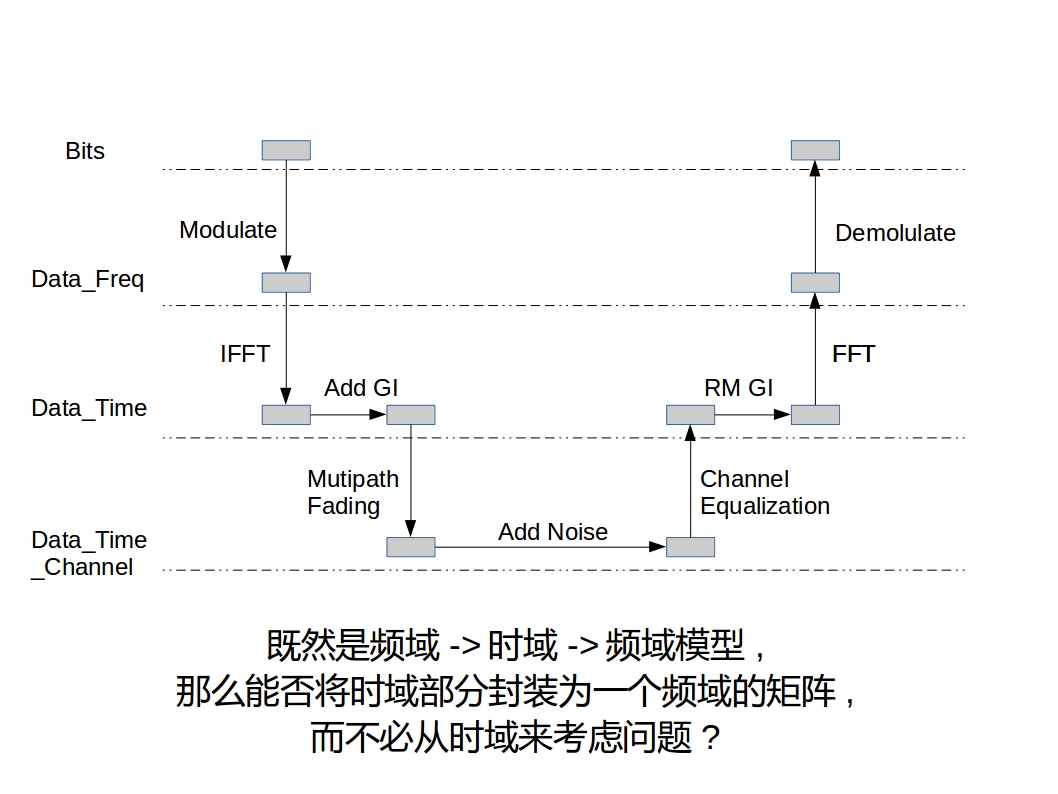
\includegraphics[width=\textwidth]{figure/top.jpg}
	\end{figure}
  \end{frame}
  \begin{frame}{整体框架--数学描述}
	\begin{equation*}
	  \begin{aligned}
	\hat Y &= FHF^{-1}X+FW \\
	 Y &= \hat Y * \frac{H_0^*}{||H_0||^2}\\
	 H_0 &= \frac{P_{Re}}{P_{Tr}} \\
	  \end{aligned}
	\end{equation*}
  \end{frame}

  \section{数字实现}
  \begin{frame}{数字实现---信道矩阵}
	\\方法一:加循环前缀和循环延时
	\scalebox{0.5}{ 	\begin{equation*}
	  \begin{aligned}
		HX &= \\ &
		\begin{pmatrix}
		 h(Q-1)&\ldots  &h(0)  & \ldots  & 0 & 0 & 0  & \ldots & 0 \\ 
		 0&h(Q-1)&\ldots  &h(0)  & \ldots  & 0 & 0 & 0  & \ldots  \\ 
		 \ldots&0&h(Q-1)&\ldots  &h(0)  & \ldots  & 0 & 0 & 0    \\ 
		0& \ldots&0&h(Q-1)&\ldots  &h(0)  & \ldots  & 0 & 0     \\ 
		0&0& \ldots&0&h(Q-1)&\ldots  &h(0)  & \ldots  & 0      \\ 
		0&0&0& \ldots&0&h(Q-1)&\ldots  &h(0)  & \ldots        \\ 
		\ldots&0&0&0& \ldots&0&h(Q-1)&\ldots  &h(0)   \\ 
		 \end{pmatrix}
		\times 
		\begin{pmatrix}
		X(-N_{CP}-Q+1)\\ 
		\ldots\\ 
		X(-N_{CP})\\ 
		\ldots\\ 
		-1\\ 
		0\\ 
		1\\
		\ldots\\
		N\\
		\end{pmatrix}
		\\&
	if \; $n<0$, then \; X(n)=X(n+N)
	  \end{aligned}
	\end{equation*}

 }
	\\方法二:由于循环矩阵的特性, 在矩阵运算中可以将其省略
	\scalebox{0.5}{ \begin{equation*}
  \begin{aligned}
	HX&=\\ &
\begin{pmatrix}
h(0) & 0 & \ldots & h(Q-1) & \ldots & h(1)\\ 
h(1)&h(0) & 0 & \ldots & h(Q-1) & \ldots \\ 
\ldots &h(1)&h(0) & 0 & \ldots & h(Q-1) \\ 
h(Q-1)&\ldots &h(1)&h(0) & 0 & \ldots  \\ 
\ldots&h(Q-1)&\ldots &h(1)&h(0) & 0  \\ 
0&\ldots&h(Q-1)&\ldots &h(1)&h(0)   \\ 
\end{pmatrix}
\times 
\begin{pmatrix}
X(0)\\ 
X(1)\\
\ldots\\
\ldots\\
\ldots\\
\ldots\\
X(N)\\

\end{pmatrix}
  \end{aligned}
\end{equation*}
 }
  \end{frame}
  \begin{frame}{数字实现--- $F, F^{-1}, W$ }
	\begin{equation*}
  \begin{aligned}
	F&=e^{(-j 2\pi (k-1)(n-1)/N)}\\
	F^{-1}&=e^{(j 2\pi (k-1)(n-1)/N)}\\
	W &= randn()*NoisePower
  \end{aligned}
\end{equation*}

  \end{frame}
  \begin{frame}{数字实现--- 主函数 }
	\documentclass[UTF8]{ctexbeamer}
\usefonttheme[onlymath]{serif}
\usepackage{listings}  
\usepackage{fontspec}  
\setmonofont{Consolas}  
\usepackage{graphicx}
\usepackage{amsmath}
\usetheme{metropolis}           % Use metropolis theme
\title{ODFM频域模型验证}
\date{\today}
\author{李昊}
\institute{通信系统仿真大作业}
\begin{document}
  \maketitle
  \section{整体框架}
  \begin{frame}{整体框架--流程描述}
	\begin{figure}
	  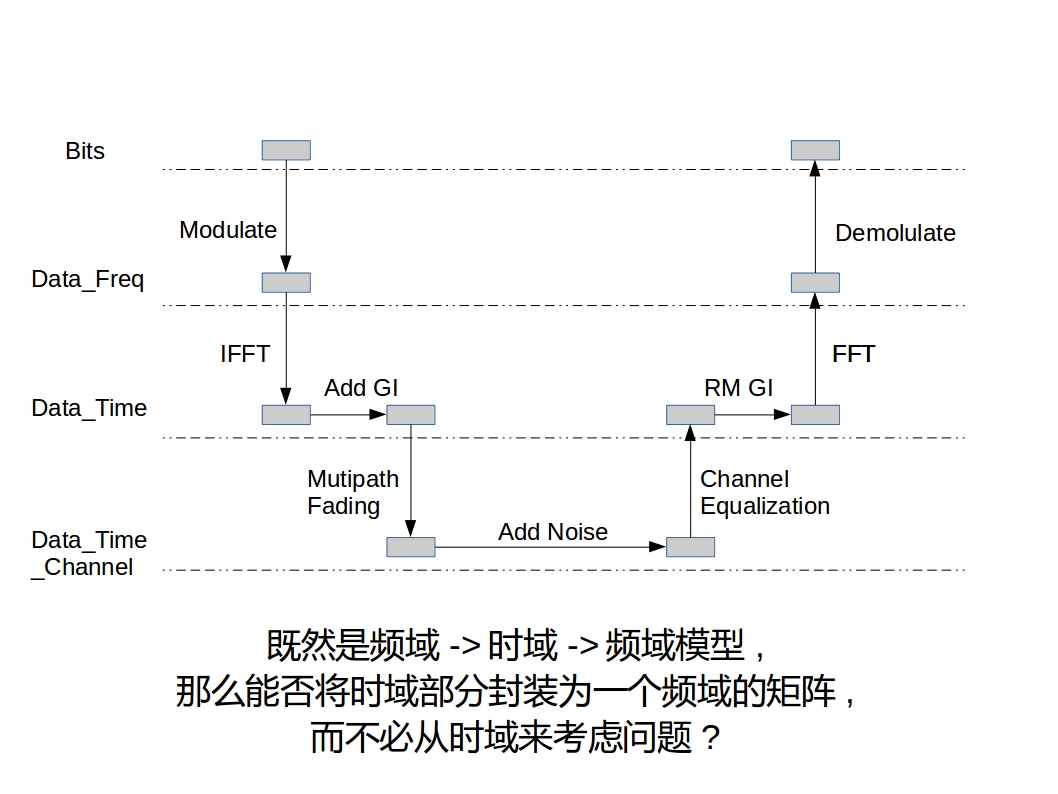
\includegraphics[width=\textwidth]{figure/top.jpg}
	\end{figure}
  \end{frame}
  \begin{frame}{整体框架--数学描述}
	\begin{equation*}
	  \begin{aligned}
	\hat Y &= FHF^{-1}X+FW \\
	 Y &= \hat Y * \frac{H_0^*}{||H_0||^2}\\
	 H_0 &= \frac{P_{Re}}{P_{Tr}} \\
	  \end{aligned}
	\end{equation*}
  \end{frame}

  \section{数字实现}
  \begin{frame}{数字实现---信道矩阵}
	\\方法一:加循环前缀和循环延时
	\scalebox{0.5}{ 	\begin{equation*}
	  \begin{aligned}
		HX &= \\ &
		\begin{pmatrix}
		 h(Q-1)&\ldots  &h(0)  & \ldots  & 0 & 0 & 0  & \ldots & 0 \\ 
		 0&h(Q-1)&\ldots  &h(0)  & \ldots  & 0 & 0 & 0  & \ldots  \\ 
		 \ldots&0&h(Q-1)&\ldots  &h(0)  & \ldots  & 0 & 0 & 0    \\ 
		0& \ldots&0&h(Q-1)&\ldots  &h(0)  & \ldots  & 0 & 0     \\ 
		0&0& \ldots&0&h(Q-1)&\ldots  &h(0)  & \ldots  & 0      \\ 
		0&0&0& \ldots&0&h(Q-1)&\ldots  &h(0)  & \ldots        \\ 
		\ldots&0&0&0& \ldots&0&h(Q-1)&\ldots  &h(0)   \\ 
		 \end{pmatrix}
		\times 
		\begin{pmatrix}
		X(-N_{CP}-Q+1)\\ 
		\ldots\\ 
		X(-N_{CP})\\ 
		\ldots\\ 
		-1\\ 
		0\\ 
		1\\
		\ldots\\
		N\\
		\end{pmatrix}
		\\&
	if \; $n<0$, then \; X(n)=X(n+N)
	  \end{aligned}
	\end{equation*}

 }
	\\方法二:由于循环矩阵的特性, 在矩阵运算中可以将其省略
	\scalebox{0.5}{ \begin{equation*}
  \begin{aligned}
	HX&=\\ &
\begin{pmatrix}
h(0) & 0 & \ldots & h(Q-1) & \ldots & h(1)\\ 
h(1)&h(0) & 0 & \ldots & h(Q-1) & \ldots \\ 
\ldots &h(1)&h(0) & 0 & \ldots & h(Q-1) \\ 
h(Q-1)&\ldots &h(1)&h(0) & 0 & \ldots  \\ 
\ldots&h(Q-1)&\ldots &h(1)&h(0) & 0  \\ 
0&\ldots&h(Q-1)&\ldots &h(1)&h(0)   \\ 
\end{pmatrix}
\times 
\begin{pmatrix}
X(0)\\ 
X(1)\\
\ldots\\
\ldots\\
\ldots\\
\ldots\\
X(N)\\

\end{pmatrix}
  \end{aligned}
\end{equation*}
 }
  \end{frame}
  \begin{frame}{数字实现--- $F, F^{-1}, W$ }
	\begin{equation*}
  \begin{aligned}
	F&=e^{(-j 2\pi (k-1)(n-1)/N)}\\
	F^{-1}&=e^{(j 2\pi (k-1)(n-1)/N)}\\
	W &= randn()*NoisePower
  \end{aligned}
\end{equation*}

  \end{frame}
  \begin{frame}{数字实现--- 主函数 }
	\documentclass[UTF8]{ctexbeamer}
\usefonttheme[onlymath]{serif}
\usepackage{listings}  
\usepackage{fontspec}  
\setmonofont{Consolas}  
\usepackage{graphicx}
\usepackage{amsmath}
\usetheme{metropolis}           % Use metropolis theme
\title{ODFM频域模型验证}
\date{\today}
\author{李昊}
\institute{通信系统仿真大作业}
\begin{document}
  \maketitle
  \section{整体框架}
  \begin{frame}{整体框架--流程描述}
	\begin{figure}
	  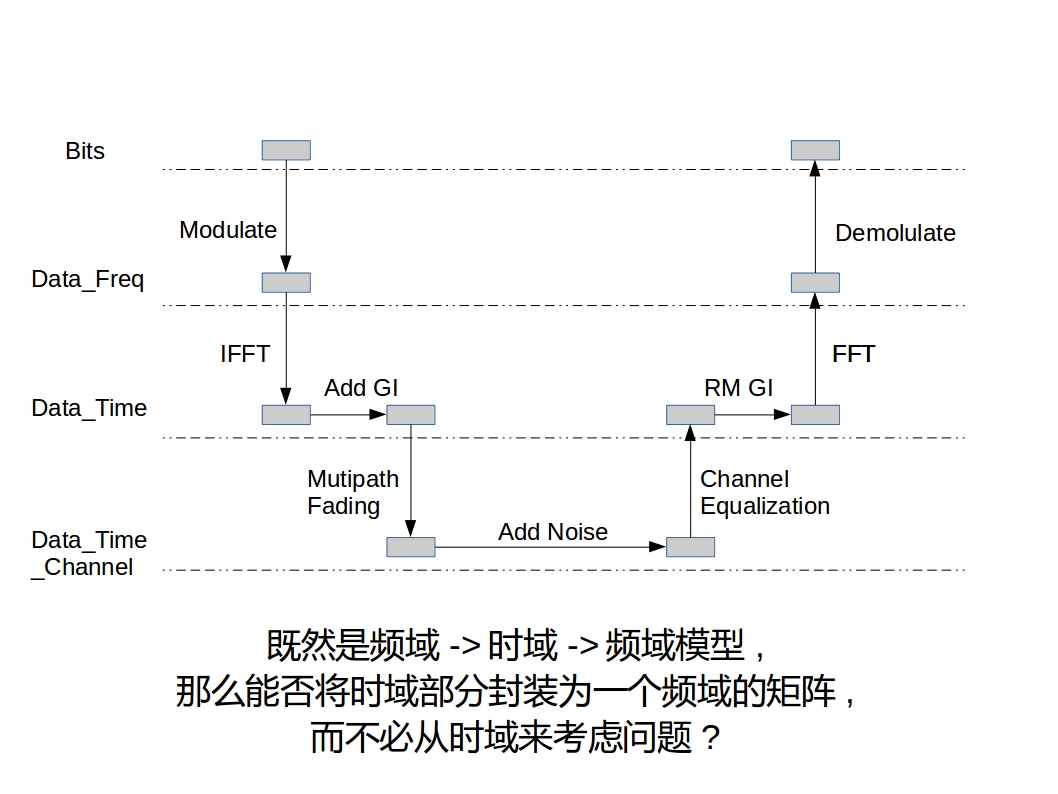
\includegraphics[width=\textwidth]{figure/top.jpg}
	\end{figure}
  \end{frame}
  \begin{frame}{整体框架--数学描述}
	\begin{equation*}
	  \begin{aligned}
	\hat Y &= FHF^{-1}X+FW \\
	 Y &= \hat Y * \frac{H_0^*}{||H_0||^2}\\
	 H_0 &= \frac{P_{Re}}{P_{Tr}} \\
	  \end{aligned}
	\end{equation*}
  \end{frame}

  \section{数字实现}
  \begin{frame}{数字实现---信道矩阵}
	\\方法一:加循环前缀和循环延时
	\scalebox{0.5}{ \input{math/H_old} }
	\\方法二:由于循环矩阵的特性, 在矩阵运算中可以将其省略
	\scalebox{0.5}{ \input{math/H_new} }
  \end{frame}
  \begin{frame}{数字实现--- $F, F^{-1}, W$ }
	\input{math/FW}
  \end{frame}
  \begin{frame}{数字实现--- 主函数 }
	\input{code/main}
  \end{frame}
  \begin{frame}{数字实现--- 方法二 }
	\input{code/way_matrix}
  \end{frame}
  \begin{frame}{数字实现--- 方法一 }
	\input{code/way_matrix_old}
  \end{frame}
  \section{结果分析}
  \begin{frame}{结果分析}
	\begin{figure}
	  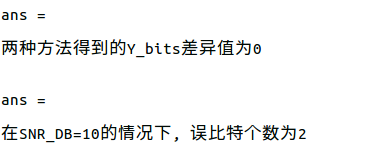
\includegraphics[width=\textwidth]{figure/result.png}
	\end{figure}
	\begin{enumerate}
	  \item 两种方法得到的结果一致, 符合预期
	  \item	效果相同, 但是方法二明显更加节省资源
	\end{enumerate}
  \end{frame}
  \begin{frame}{最后要说的话---广告时间}
	\begin{itemsize}
	  \item 感谢老师同学们的耐心帮助
	  \item	\url{https://github.com/lihao2333/mtheme/tree/ofdm}
	  \item	\url{https://github.com/lihao2333/TP_TelSimulation/tree/ofdm}
	  \item 期待你的follow和star
	\end{itemsize}

  \end{frame}
\end{document}

  \end{frame}
  \begin{frame}{数字实现--- 方法二 }
	
\begin{lstlisting}[language = matlab, numbers=left, \fontsize{6pt}{8pt}, 
        numberstyle=\tiny,keywordstyle=\color{blue!70},  breaklines=true,tabsize=2,
        commentstyle=\color{red!50!green!50!blue!50},frame=shadowbox,  
        rulesepcolor=\color{red!20!green!20!blue!20},basicstyle=\ttfamily]  

%% 通过矩阵的方式完成一个frame的ofdm, 输入和输出都是调制信号
%	input:
%		X:	调制后的发送信号, 格式为[preamble, x1, x2...], preamble, xn 都是列向量
%		H:	信道矩阵
%		W:噪声矩阵
%	output:
%		Y:	输出序列
function Y = way_matrix(X, H,  W)
	[NumCarry, NumSymble] = size(X);
	[F, Fi] = gen_F(NumCarry);
	Y = F*(H*(Fi*(X)))+F*W;
	Hi = Y(:,1)./X(:,1);
	Hi = repmat(Hi,[1,NumSymble]);
	Y = Y./Hi;
end
 \end{lstlisting}  

  \end{frame}
  \begin{frame}{数字实现--- 方法一 }
	
\begin{lstlisting}[language = matlab, numbers=left, \fontsize{6pt}{8pt}, 
        numberstyle=\tiny,keywordstyle=\color{blue!70},  tabsize=2,
        commentstyle=\color{red!50!green!50!blue!50},frame=shadowbox,  breaklines=true,
        rulesepcolor=\color{red!20!green!20!blue!20},basicstyle=\ttfamily]  

%% 通过矩阵的方式完成一个frame的ofdm, 输入和输出都是调制信号
%	input:
%		X:	调制后的发送信号, 格式为[preamble, x1, x2...], preamble, xn 都是列向量
%		H:	信道矩阵
%		W:噪声矩阵
%	output:
%		Y:	输出序列
function Y = way_matrix_old(X, H,  W, NumCP, MaxDelay)
	[F, Fi] = gen_F(size(W,1));
	X_time = (Fi*(X));
	X_time_CP_Delay = [X_time(end-(NumCP+MaxDelay-1):end,:);X_time];
	X_time_CP_H = H*X_time_CP_Delay ;
	X_time_H_W = X_time_CP_H(1+(NumCP):end,:)+W;
	Y = F*X_time_H_W;
	Hi = Y(:,1)./X(:,1);
	Hi = repmat(Hi,[1,size(X,2)]);
	Y = Y./Hi;
end
 \end{lstlisting}  

  \end{frame}
  \section{结果分析}
  \begin{frame}{结果分析}
	\begin{figure}
	  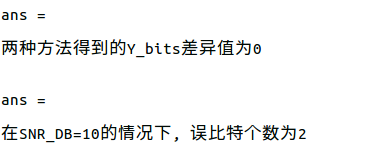
\includegraphics[width=\textwidth]{figure/result.png}
	\end{figure}
	\begin{enumerate}
	  \item 两种方法得到的结果一致, 符合预期
	  \item	效果相同, 但是方法二明显更加节省资源
	\end{enumerate}
  \end{frame}
  \begin{frame}{最后要说的话---广告时间}
	\begin{itemsize}
	  \item 感谢老师同学们的耐心帮助
	  \item	\url{https://github.com/lihao2333/mtheme/tree/ofdm}
	  \item	\url{https://github.com/lihao2333/TP_TelSimulation/tree/ofdm}
	  \item 期待你的follow和star
	\end{itemsize}

  \end{frame}
\end{document}

  \end{frame}
  \begin{frame}{数字实现--- 方法二 }
	
\begin{lstlisting}[language = matlab, numbers=left, \fontsize{6pt}{8pt}, 
        numberstyle=\tiny,keywordstyle=\color{blue!70},  breaklines=true,tabsize=2,
        commentstyle=\color{red!50!green!50!blue!50},frame=shadowbox,  
        rulesepcolor=\color{red!20!green!20!blue!20},basicstyle=\ttfamily]  

%% 通过矩阵的方式完成一个frame的ofdm, 输入和输出都是调制信号
%	input:
%		X:	调制后的发送信号, 格式为[preamble, x1, x2...], preamble, xn 都是列向量
%		H:	信道矩阵
%		W:噪声矩阵
%	output:
%		Y:	输出序列
function Y = way_matrix(X, H,  W)
	[NumCarry, NumSymble] = size(X);
	[F, Fi] = gen_F(NumCarry);
	Y = F*(H*(Fi*(X)))+F*W;
	Hi = Y(:,1)./X(:,1);
	Hi = repmat(Hi,[1,NumSymble]);
	Y = Y./Hi;
end
 \end{lstlisting}  

  \end{frame}
  \begin{frame}{数字实现--- 方法一 }
	
\begin{lstlisting}[language = matlab, numbers=left, \fontsize{6pt}{8pt}, 
        numberstyle=\tiny,keywordstyle=\color{blue!70},  tabsize=2,
        commentstyle=\color{red!50!green!50!blue!50},frame=shadowbox,  breaklines=true,
        rulesepcolor=\color{red!20!green!20!blue!20},basicstyle=\ttfamily]  

%% 通过矩阵的方式完成一个frame的ofdm, 输入和输出都是调制信号
%	input:
%		X:	调制后的发送信号, 格式为[preamble, x1, x2...], preamble, xn 都是列向量
%		H:	信道矩阵
%		W:噪声矩阵
%	output:
%		Y:	输出序列
function Y = way_matrix_old(X, H,  W, NumCP, MaxDelay)
	[F, Fi] = gen_F(size(W,1));
	X_time = (Fi*(X));
	X_time_CP_Delay = [X_time(end-(NumCP+MaxDelay-1):end,:);X_time];
	X_time_CP_H = H*X_time_CP_Delay ;
	X_time_H_W = X_time_CP_H(1+(NumCP):end,:)+W;
	Y = F*X_time_H_W;
	Hi = Y(:,1)./X(:,1);
	Hi = repmat(Hi,[1,size(X,2)]);
	Y = Y./Hi;
end
 \end{lstlisting}  

  \end{frame}
  \section{结果分析}
  \begin{frame}{结果分析}
	\begin{figure}
	  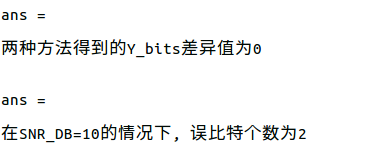
\includegraphics[width=\textwidth]{figure/result.png}
	\end{figure}
	\begin{enumerate}
	  \item 两种方法得到的结果一致, 符合预期
	  \item	效果相同, 但是方法二明显更加节省资源
	\end{enumerate}
  \end{frame}
  \begin{frame}{最后要说的话---广告时间}
	\begin{itemsize}
	  \item 感谢老师同学们的耐心帮助
	  \item	\url{https://github.com/lihao2333/mtheme/tree/ofdm}
	  \item	\url{https://github.com/lihao2333/TP_TelSimulation/tree/ofdm}
	  \item 期待你的follow和star
	\end{itemsize}

  \end{frame}
\end{document}

  \end{frame}
  \begin{frame}{数字实现--- 方法二 }
	
\begin{lstlisting}[language = matlab, numbers=left, \fontsize{6pt}{8pt}, 
        numberstyle=\tiny,keywordstyle=\color{blue!70},  breaklines=true,tabsize=2,
        commentstyle=\color{red!50!green!50!blue!50},frame=shadowbox,  
        rulesepcolor=\color{red!20!green!20!blue!20},basicstyle=\ttfamily]  

%% 通过矩阵的方式完成一个frame的ofdm, 输入和输出都是调制信号
%	input:
%		X:	调制后的发送信号, 格式为[preamble, x1, x2...], preamble, xn 都是列向量
%		H:	信道矩阵
%		W:噪声矩阵
%	output:
%		Y:	输出序列
function Y = way_matrix(X, H,  W)
	[NumCarry, NumSymble] = size(X);
	[F, Fi] = gen_F(NumCarry);
	Y = F*(H*(Fi*(X)))+F*W;
	Hi = Y(:,1)./X(:,1);
	Hi = repmat(Hi,[1,NumSymble]);
	Y = Y./Hi;
end
 \end{lstlisting}  

  \end{frame}
  \begin{frame}{数字实现--- 方法一 }
	
\begin{lstlisting}[language = matlab, numbers=left, \fontsize{6pt}{8pt}, 
        numberstyle=\tiny,keywordstyle=\color{blue!70},  tabsize=2,
        commentstyle=\color{red!50!green!50!blue!50},frame=shadowbox,  breaklines=true,
        rulesepcolor=\color{red!20!green!20!blue!20},basicstyle=\ttfamily]  

%% 通过矩阵的方式完成一个frame的ofdm, 输入和输出都是调制信号
%	input:
%		X:	调制后的发送信号, 格式为[preamble, x1, x2...], preamble, xn 都是列向量
%		H:	信道矩阵
%		W:噪声矩阵
%	output:
%		Y:	输出序列
function Y = way_matrix_old(X, H,  W, NumCP, MaxDelay)
	[F, Fi] = gen_F(size(W,1));
	X_time = (Fi*(X));
	X_time_CP_Delay = [X_time(end-(NumCP+MaxDelay-1):end,:);X_time];
	X_time_CP_H = H*X_time_CP_Delay ;
	X_time_H_W = X_time_CP_H(1+(NumCP):end,:)+W;
	Y = F*X_time_H_W;
	Hi = Y(:,1)./X(:,1);
	Hi = repmat(Hi,[1,size(X,2)]);
	Y = Y./Hi;
end
 \end{lstlisting}  

  \end{frame}
  \section{结果分析}
  \begin{frame}{结果分析}
	\begin{figure}
	  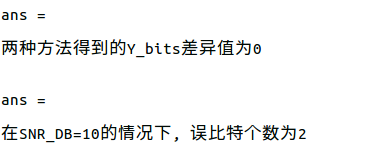
\includegraphics[width=\textwidth]{figure/result.png}
	\end{figure}
	\begin{enumerate}
	  \item 两种方法得到的结果一致, 符合预期
	  \item	效果相同, 但是方法二明显更加节省资源
	\end{enumerate}
  \end{frame}
  \begin{frame}{最后要说的话---广告时间}
	\begin{itemsize}
	  \item 感谢老师同学们的耐心帮助
	  \item	\url{https://github.com/lihao2333/mtheme/tree/ofdm}
	  \item	\url{https://github.com/lihao2333/TP_TelSimulation/tree/ofdm}
	  \item 期待你的follow和star
	\end{itemsize}

  \end{frame}
\end{document}
